%%%%%%%%%%%%%%%%%%%%%%%%%%%%%%%%%%%%
% Lesson Plan (50 minutes)
%%%%%%%%%%%%%%%%%%%%%%%%%%%%%%%%%%%%
\begin{frame}
    \frametitle{Lesson Plan}
    \begin{itemize}
        \item xx min Lecture: Motivate linear regression, modeling numerical variables
        \item xx min R Demonstration: scatter plots, response/explanatory variable(s), determining relationships
        \item xx min Edfinity quiz: from scatter plots, practice determining response/explanatory and relationship between variables for different examples
        \item xx min Lecture: residuals, correlation
        \item xx min Edfinity quiz: guessing and then assessing correlation (like slides 10-11)
        \item xx min Lecture: motivate line-fitting (next time)
    \end{itemize}
\end{frame}

%%%%%%%%%%%%%%%%%%%%%%%%%%%%%%%%%%%%
% Learning objectives:
%%%%%%%%%%%%%%%%%%%%%%%%%%%%%%%%%%%%
\begin{frame}
    \frametitle{Learning Objectives}
    \begin{itemize}
        \item \textbf{M1, LO1: Classify and Analyze Variables:} Categorize variables based on their types (e.g., numerical/categorical, continuous/discrete, ordinal), assess their association (positive, negative, or independent), and determine which make sense as explanatory vs. response variables.
        \item \textbf{M1, LO3: Use R for Data Management and Exploration:} Utilize R to load, pre-process, and explore data through visualization and summarization techniques.
        \item \textbf{M1, LO4: Visualize and Describe Data Distributions:} Select appropriate visualizations (scatterplots, histograms, box plots, bar plots) to depict data, and describe distributions qualitatively (shape, center, spread, outliers) and quantitatively (mean, median, mode, range, IQR, standard deviation).
        \item \textbf{M5, LO1: Describe and Assess Relationships Between Two Variables:} Describe the association between two numerical variables in a scatter plot in terms of direction, shape (linear or nonlinear), and strength, and assess whether linear regression is an appropriate model.    
    \end{itemize}
\end{frame}
    
%%%%%%%%%%%%%%%%%%%%%%%%%%%%%%%%%%%%
% TODO: Copy and adapt these slides base on the lesson plan
%%%%%%%%%%%%%%%%%%%%%%%%%%%%%%%%%%%%

\section{Line fitting, residuals, and correlation}

%%%%%%%%%%%%%%%%%%%%%%%%%%%%%%%%%%%%

\subsection{Fitting a line to data}

%%%%%%%%%%%%%%%%%%%%%%%%%%%%%%%%%%%%

\begin{frame}
\frametitle{Modeling numerical variables}

In this unit we will learn to quantify the relationship between two numerical variables, as well as modeling numerical response variables using a numerical or categorical explanatory variable.

\end{frame}

%%%%%%%%%%%%%%%%%%%%%%%%%%%%%%%%%%%%

\begin{frame}
\frametitle{Poverty vs. HS graduate rate}

The \hl{scatterplot} below shows the relationship between HS graduate rate in all 50 US states and DC and the \% of residents who live below the poverty line {\small (income below \$23,050 for a family of 4 in 2012)}.

\twocol{0.55}{0.45}{
\begin{center}
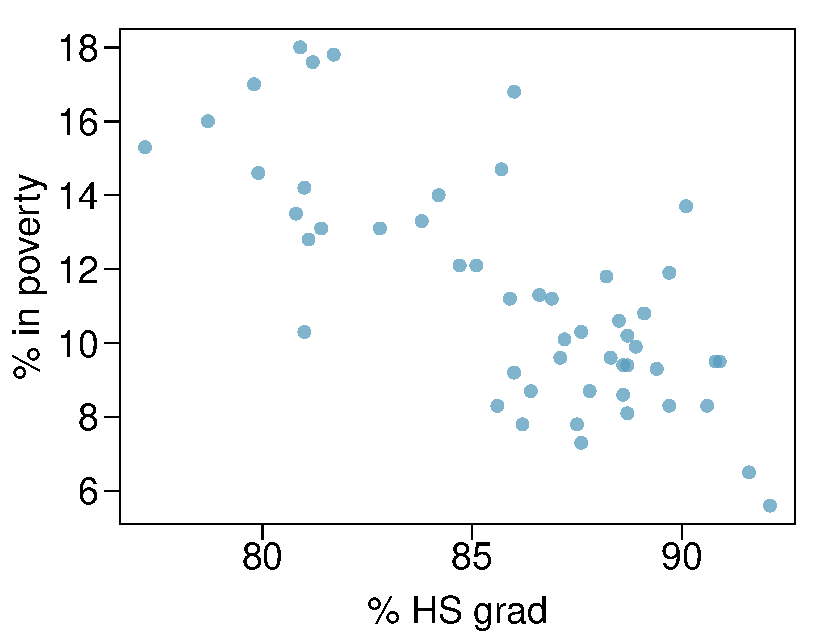
\includegraphics[width=\textwidth]{8-1_linefit_res_corr/figures/poverty/poverty_hsgrad}
\end{center}
}
{
\dq{Response variable?}
\pause
\soln{\% in poverty}
\pause
\dq{Explanatory variable?}
\pause
\soln{\% HS grad}
\pause
\dq{Relationship?}
\pause
\soln{linear, negative, moderately strong}
}

\end{frame}

%%%%%%%%%%%%%%%%%%%%%%%%%%%%%%%%%%%

\subsection{Using a linear regression to predict poverty}

%%%%%%%%%%%%%%%%%%%%%%%%%%%%%%%%%%%

\begin{frame}

The linear model for predicting poverty from high school graduation rate in the US is

\[ \hat{poverty} = 64.78 - 0.62 * HS_{grad} \]

The ``hat" is used to signify that this is an estimate.

\end{frame}

%%%%%%%%%%%%%%%%%%%%%%%%%%%%%%%%%%%

\begin{frame}

\dq{The high school graduate rate in Georgia is 85.1\%. What poverty level does the model predict for this state?}

\pause

\[ 64.78 - 0.62 * 85.1 = 12.018 \]

\end{frame}

%%%%%%%%%%%%%%%%%%%%%%%%%%%%%%%%%%%

\subsection{Eyeballing the line}

%%%%%%%%%%%%%%%%%%%%%%%%%%%%%%%%%%%

\begin{frame}
\frametitle{Eyeballing the line}

\twocol{0.3}{0.7}
{
\pq{Which of the following appears to be the line that best fits the linear relationship between \% in poverty and \% HS grad? Choose one.}
\soln{\only<2>{\orange{
(a)
}}}
}
{
\begin{center}
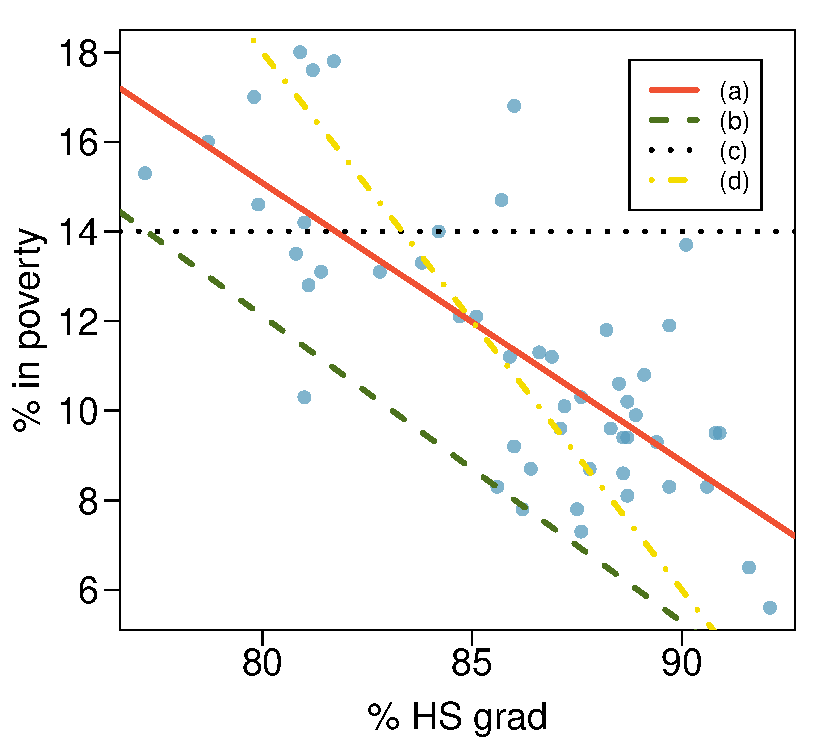
\includegraphics[width=\textwidth]{8-2_least_square_reg/figures/poverty/poverty_hsgrad_manylines}
\end{center}
}
\end{frame}

%%%%%%%%%%%%%%%%%%%%%%%%%%%%%%%%%%%

\subsection{Residuals}

%%%%%%%%%%%%%%%%%%%%%%%%%%%%%%%%%%%

\begin{frame}
\frametitle{Residuals}

\hl{Residuals} are the leftovers from the model fit: Data = Fit + Residual

\begin{center}
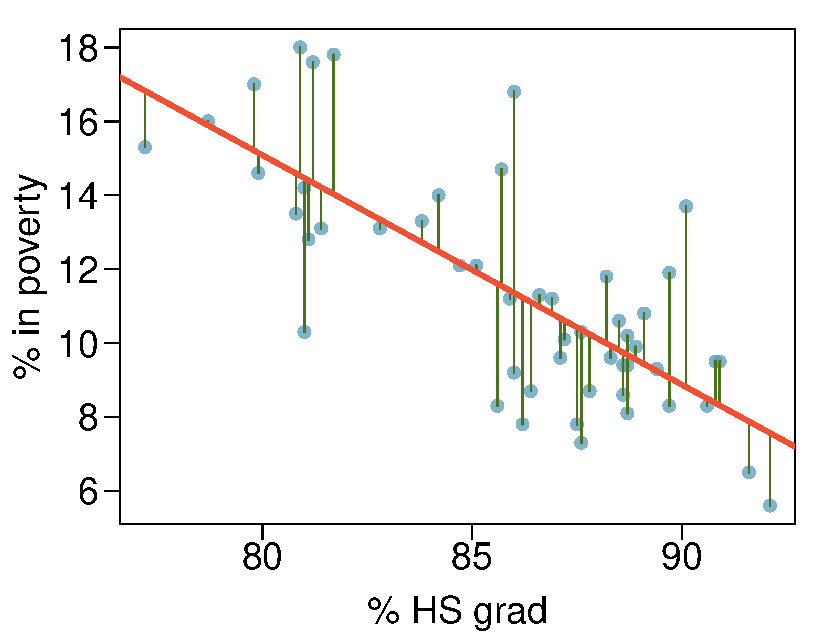
\includegraphics[width=0.8\textwidth]{8-2_least_square_reg/figures/poverty/poverty_hsgrad_res}
\end{center}

\end{frame}

%%%%%%%%%%%%%%%%%%%%%%%%%%%%%%%%%%

\begin{frame}
\frametitle{Residuals (cont.)}

\formula{Residual}{
Residual is the difference between the observed ($y_i$) and predicted $\hat{y}_i$. 
\[ e_i = y_i - \hat{y}_i \]
}
\vspace{-0.5cm}
\twocol{0.6}{0.4}
{
\begin{center}
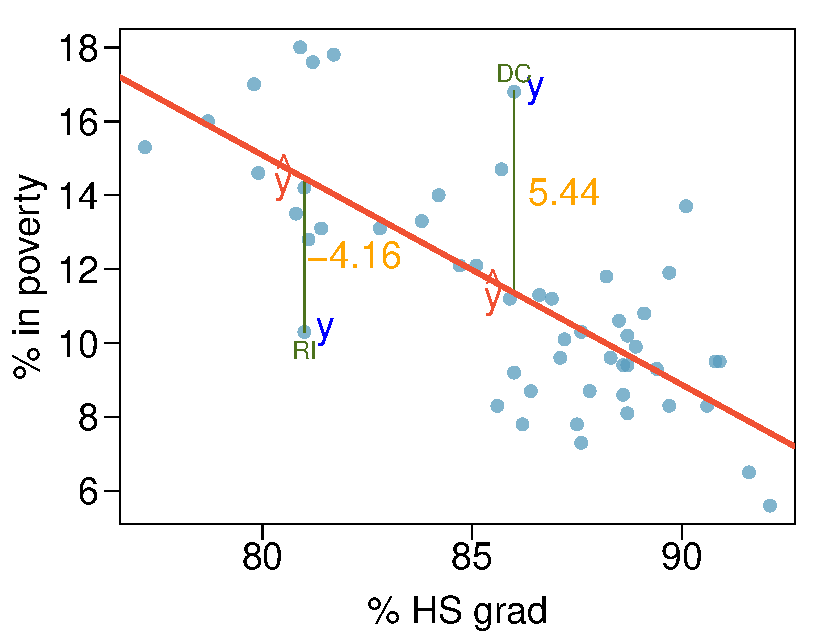
\includegraphics[width=\textwidth]{8-2_least_square_reg/figures/poverty/poverty_hsgrad_res_text}
\end{center}
}
{
\pause
\begin{itemize}
\item \% living in poverty in DC is 5.44\% more than predicted.
\pause
\item \% living in poverty in RI is 4.16\% less than predicted.
\end{itemize}
}


\end{frame}

%%%%%%%%%%%%%%%%%%%%%%%%%%%%%%%%%%

\subsection{Describing linear relationships with correlation}

%%%%%%%%%%%%%%%%%%%%%%%%%%%%%%%%%%%

\begin{frame}
\frametitle{Quantifying the relationship}

\begin{itemize}

\item \hl{Correlation} describes the strength of the \orange{linear} association between two variables.

\pause

\item It takes values between -1 (perfect negative) and +1 (perfect positive).

\pause

\item A value of 0 indicates no linear association.

\end{itemize}

\end{frame}

%%%%%%%%%%%%%%%%%%%%%%%%%%%%%%%%%%%

\begin{frame}
\frametitle{Guessing the correlation}

\pq{Which of the following is the best guess for the correlation between \% in poverty and \% HS grad?}
\twocol{0.4}{0.6}
{
\begin{enumerate}[(a)]
\item 0.6
\solnMult{-0.75}
\item -0.1
\item 0.02
\item -1.5
\end{enumerate}
}
{
\begin{center}
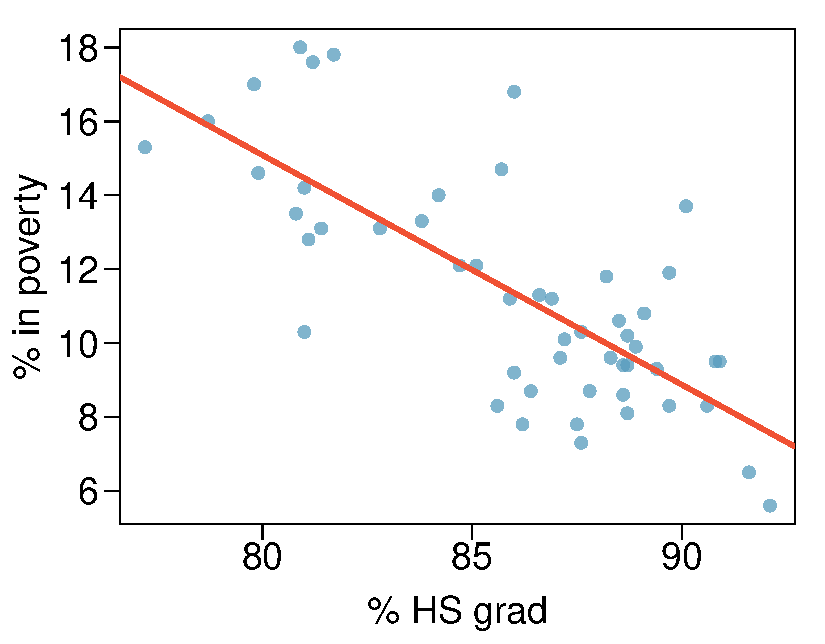
\includegraphics[width=\textwidth]{8-1_linefit_res_corr/figures/poverty/poverty_hsgrad_line}
\end{center}
}

\end{frame}

%%%%%%%%%%%%%%%%%%%%%%%%%%%%%%%%%%

\begin{frame}
\frametitle{Guessing the correlation}

\pq{Which of the following is the best guess for the correlation between \%~in~poverty and \% HS grad?}

\twocol{0.4}{0.6}
{
\begin{enumerate}[(a)]
\item 0.1
\item -0.6
\item -0.4
\item 0.9
\solnMult{0.5}
\end{enumerate}
}
{
\begin{center}
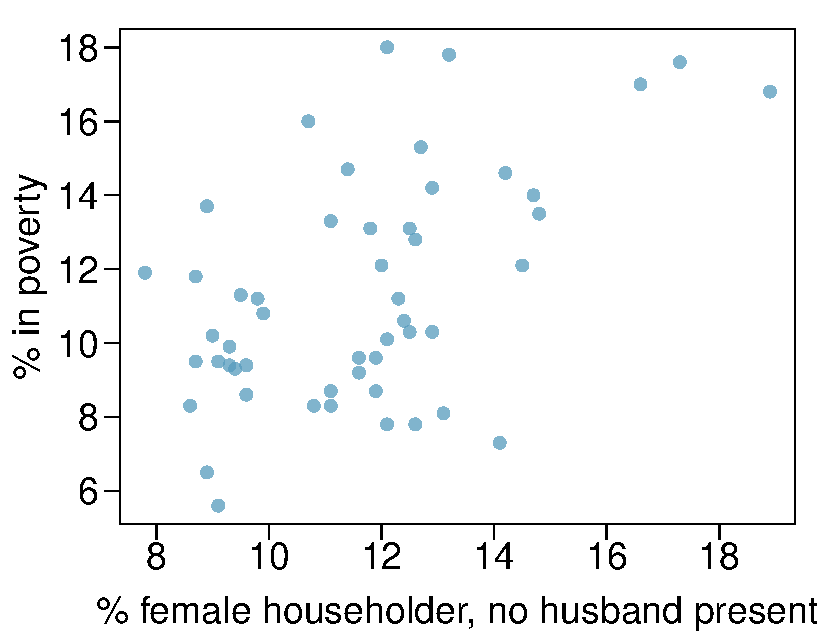
\includegraphics[width=\textwidth]{8-1_linefit_res_corr/figures/poverty/poverty_nohusband}
\end{center}
}

\end{frame}

%%%%%%%%%%%%%%%%%%%%%%%%%%%%%%%%%%

\begin{frame}
\frametitle{Assessing the correlation}

\pq{Which of the following is has the strongest correlation, i.e. correlation coefficient closest to +1 or -1?}

\twocol{0.8}{0.2}
{
\begin{center}
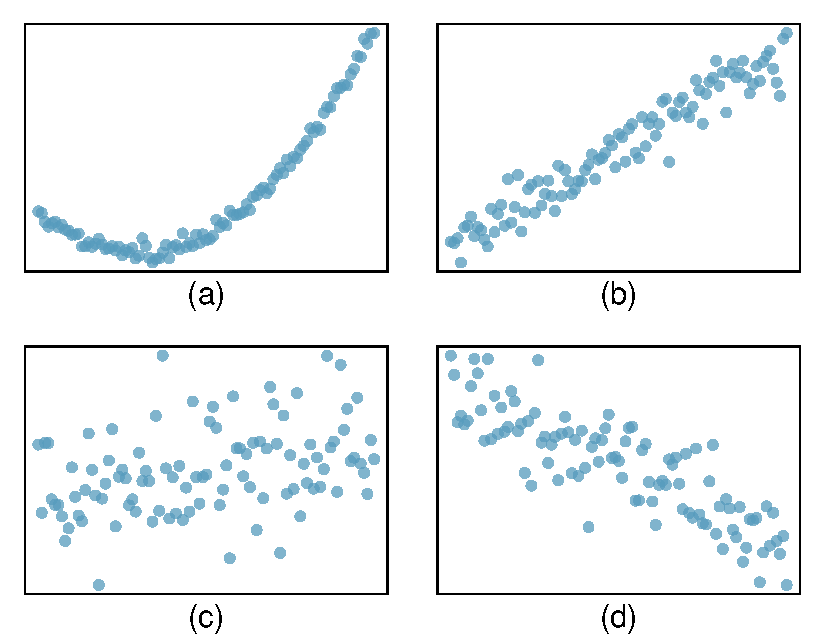
\includegraphics[width=0.75\textwidth]{8-1_linefit_res_corr/figures/cor/cor}
\end{center}
}
{
\soln{\only<2>{\orange{
(b) $\rightarrow$ correlation means \underline{linear} association
}}}
}

\end{frame}
